\documentclass[10pt,fleqn]{article}
\usepackage{/home/clair/Documents/mystyle}
\usetikzlibrary{automata,positioning}
%----------------------------------------------------------------------
% reformat section headers to be smaller \& left-aligned
\titleformat{\section}
	{\normalfont\bfseries}
	{\thesection}{1em}{}
	
\titleformat{\subsection}
	{\normalfont\bfseries}
	{\llap{\parbox{1cm}{\thesubsection}}}{0em}{}
	
%----------------------------------------------------------------------
% SPECIFY BIBLIOGRAPHY FILE & FIELDS TO EXCLUDE
%\addbibresource{bibfile.bib}
%\AtEveryBibitem{\clearfield{url}}
%\AtEveryBibitem{\clearfield{doi}}
%\AtEveryBibitem{\clearfield{isbn}}
%\AtEveryBibitem{\clearfield{issn}}

%----------------------------------------------------------------------
% define colour to match that used by R
  \definecolor{gold}{rgb}{1.0, 0.84, 0.0}
%======================================================================

\usepackage{fancyhdr}

\fancyhf{}
\fancyhead[R]{\textbf{7-Apr-2016}}
\pagestyle{fancy}

\addtolength{\topmargin}{-0.5cm}
\addtolength{\textheight}{1.4cm}

\renewcommand{\headrulewidth}{0pt}

\begin{document}

\subsection*{Quick notes}

\begin{itemize}

\item
Black images on 15-01-08 are somehow corrupted: First and last 10 images are identical (as in \texttt{all(b.150108[ , , 1] == b.150108[ , , 2]) == T, all(b.150108[ , , 11] == b.150108[ , , 12]) == T}. As a result, 14470pts have SD = 0; gives such a low mean SD that model fitting is meaningless.
 
\item Tried fitting different shapes (hyper-ellipses, including ellipse and squircle). Improvement in residual MAD/SD after panel fitting is very slight in recent images. However, suspect that in old data, spot veers closer to square, so might be useful to allow $n$ to vary with the data.

\item Fitted mini-panels: no major change to MAD and SD of residuals, but spatial distribution differs. Think this is over-fitting: edge panels on grey \& white are `tipped up' by low values along panel border, so values around row 512 are too low. Better to fit a more sophisticated spot or panel model.

\item Found another line of warm pixels: black image 14-10-09, panel L7, col 43 = [809,1:992,"black", 141009]

\end{itemize}

\subsection*{Current questions/considerations}
\begin{itemize}

\item Still more work needed on appropriate threshold setting (\& justification thereof) for bad SD. Applying same limit as for residuals picks up large numbers of apparently normal pixels.

\item Need to make clear that we cannot expect to get a perfectly-fitting model. If the panels were behaving perfectly as expected then residuals should follow distribution exactly (Johnson accounts for skew/kurtosis due to movement of mean level within finite space) - but since the distribution is bounded, we will always have clusters of high/low values, as pixels `drift' to the extremes.

\item Goodness of fit tests are meaningless for same reason: our null hypothesis expects large numbers of pixels at extremes. With such a large sample size, a small number of these extreme values will cause GoF tests to fail (could test sensitivity if necessary)
\end{itemize}

%=============================================================================================================================
\newpage
\section*{Tracking development of bad pixels over time}

Parametric model used: circular spot fitted by linear regression of value against distance from centre $z$ and $z^2$, panels fitted by linear regression over $x$, $x^2$, $y$, $y^2$ with interactions (most complex model currently considered for panel fitting). A Johnson distribution was fitted to the residuals for each image, with points $< Q_{0.001}$ labelled as \texttt{dim} and points $> Q_{0.999}$ labelled as \texttt{bright}. A Johnson distribution was fitted separately to the pixelwise SD for each image, with points $< Q_{0.0001}$ labelled as \texttt{quiet} and those $> Q_{0.9999}$ as \texttt{noisy}.

\subsection*{14-10-09}

\begin{figure}[!h]
\caption{Bad pixels identified in each image set: 
\textcolor{blue}{$\bullet$} dead; \textcolor{green}{$\bullet$} dim;  \textcolor{gold}{$\bullet$} bright; \textcolor{red}{$\bullet$} hot}
\includegraphics[scale=0.55]{../../Models/Complex-parametric/Bad-px-detected-141009.pdf}
\end{figure}


\begin{figure}[!h]
\caption{Bad SDs identified in each image set: 
\textcolor{purple}{$\bullet$} static; \textcolor{BlueViolet}{$\bullet$} quiet;  \textcolor{orange}{$\bullet$} noisy}
\includegraphics[scale=0.55]{../../Models/Complex-parametric/Bad-sd-detected-141009.pdf}
\end{figure}

\begin{footnotesize}
\begin{verbatim}
	# Quick summary of pixels identified in all images
       #        static   quiet   noisy       -
       # dead        5       0       0       0
       # dim         0     164       2    9588
       # bright      0       4    1782   10637
       # hot       131       0       0       0
       # -           0     564    2199       0
\end{verbatim}
\end{footnotesize}

\subsection*{14-11-18}
\begin{footnotesize}
\begin{verbatim}
	# Quick summary of pixels identified in all images;		
       #        static quiet noisy     -						
       # dead        5     0     0     0
       # dim         0   108     5  8609
       # bright      0     4  1642 12455
       # hot       138     0     0     0
       # -           0   268  1143     0
       
               px.is
px.was      - bright dead  dim  hot
  -      3894   4363    0 2457    0
  bright 2690   9723    0    0   10
  dead      0      0    5    0    0
  dim    3482     12    0 6260    0
  hot       0      3    0    0  128
\end{verbatim}
\end{footnotesize}

\subsection*{State diagram}



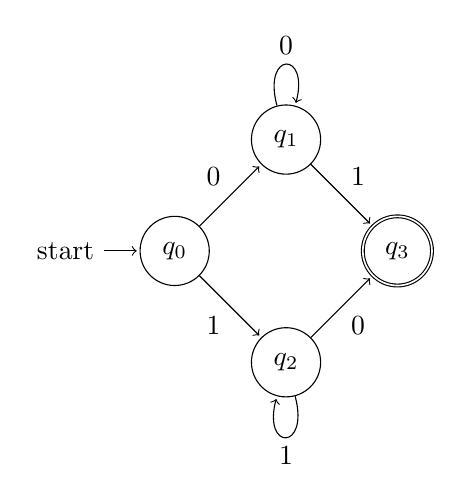
\begin{tikzpicture}[shorten >=1pt,node distance=2cm,on grid,auto] 
   \node[state,initial] (q_0)   {$q_0$}; 
   \node[state] (q_1) [above right=of q_0] {$q_1$}; 
   \node[state] (q_2) [below right=of q_0] {$q_2$}; 
   \node[state,accepting](q_3) [below right=of q_1] {$q_3$};
    \path[->] 
    (q_0) edge  node {0} (q_1)
          edge  node [swap] {1} (q_2)
    (q_1) edge  node  {1} (q_3)
          edge [loop above] node {0} ()
    (q_2) edge  node [swap] {0} (q_3) 
          edge [loop below] node {1} ();
\end{tikzpicture}
 

\end{document}